
El circuito se implementó en \textbf{PCB} de desarrollo, de las típicas de islas perforadas de paso $0.1''$, los módulos se montaron en gabinetes plásticos con ventanas para la recepción y transmisión, con los LED indicadores en el frente de cada módulo. La alimentación de ambos módulos es con una fuente de continua de $12 \si[per-mode=symbol]{\volt}$ a $16 \si[per-mode=symbol]{\volt}$, la cual se conecta con un plug standard, de modo similar el cable de interconexión se conecta con jacks de $3.5 \si[per-mode=symbol]{\milli\meter}$. \\

En las figura~\figref{fig:IR_receiver_real} y la figura~\figref{fig:IR_transmitter_real} pueden verse respectivamente el receptor y el transmisor implementados y en la figura~\figref{fig:IR_complete_real} puede verse la interconexión de ambos módulos con el cable y la conexión de alimentación.

\clearpage

\begin{figure}[H]
	\centering
	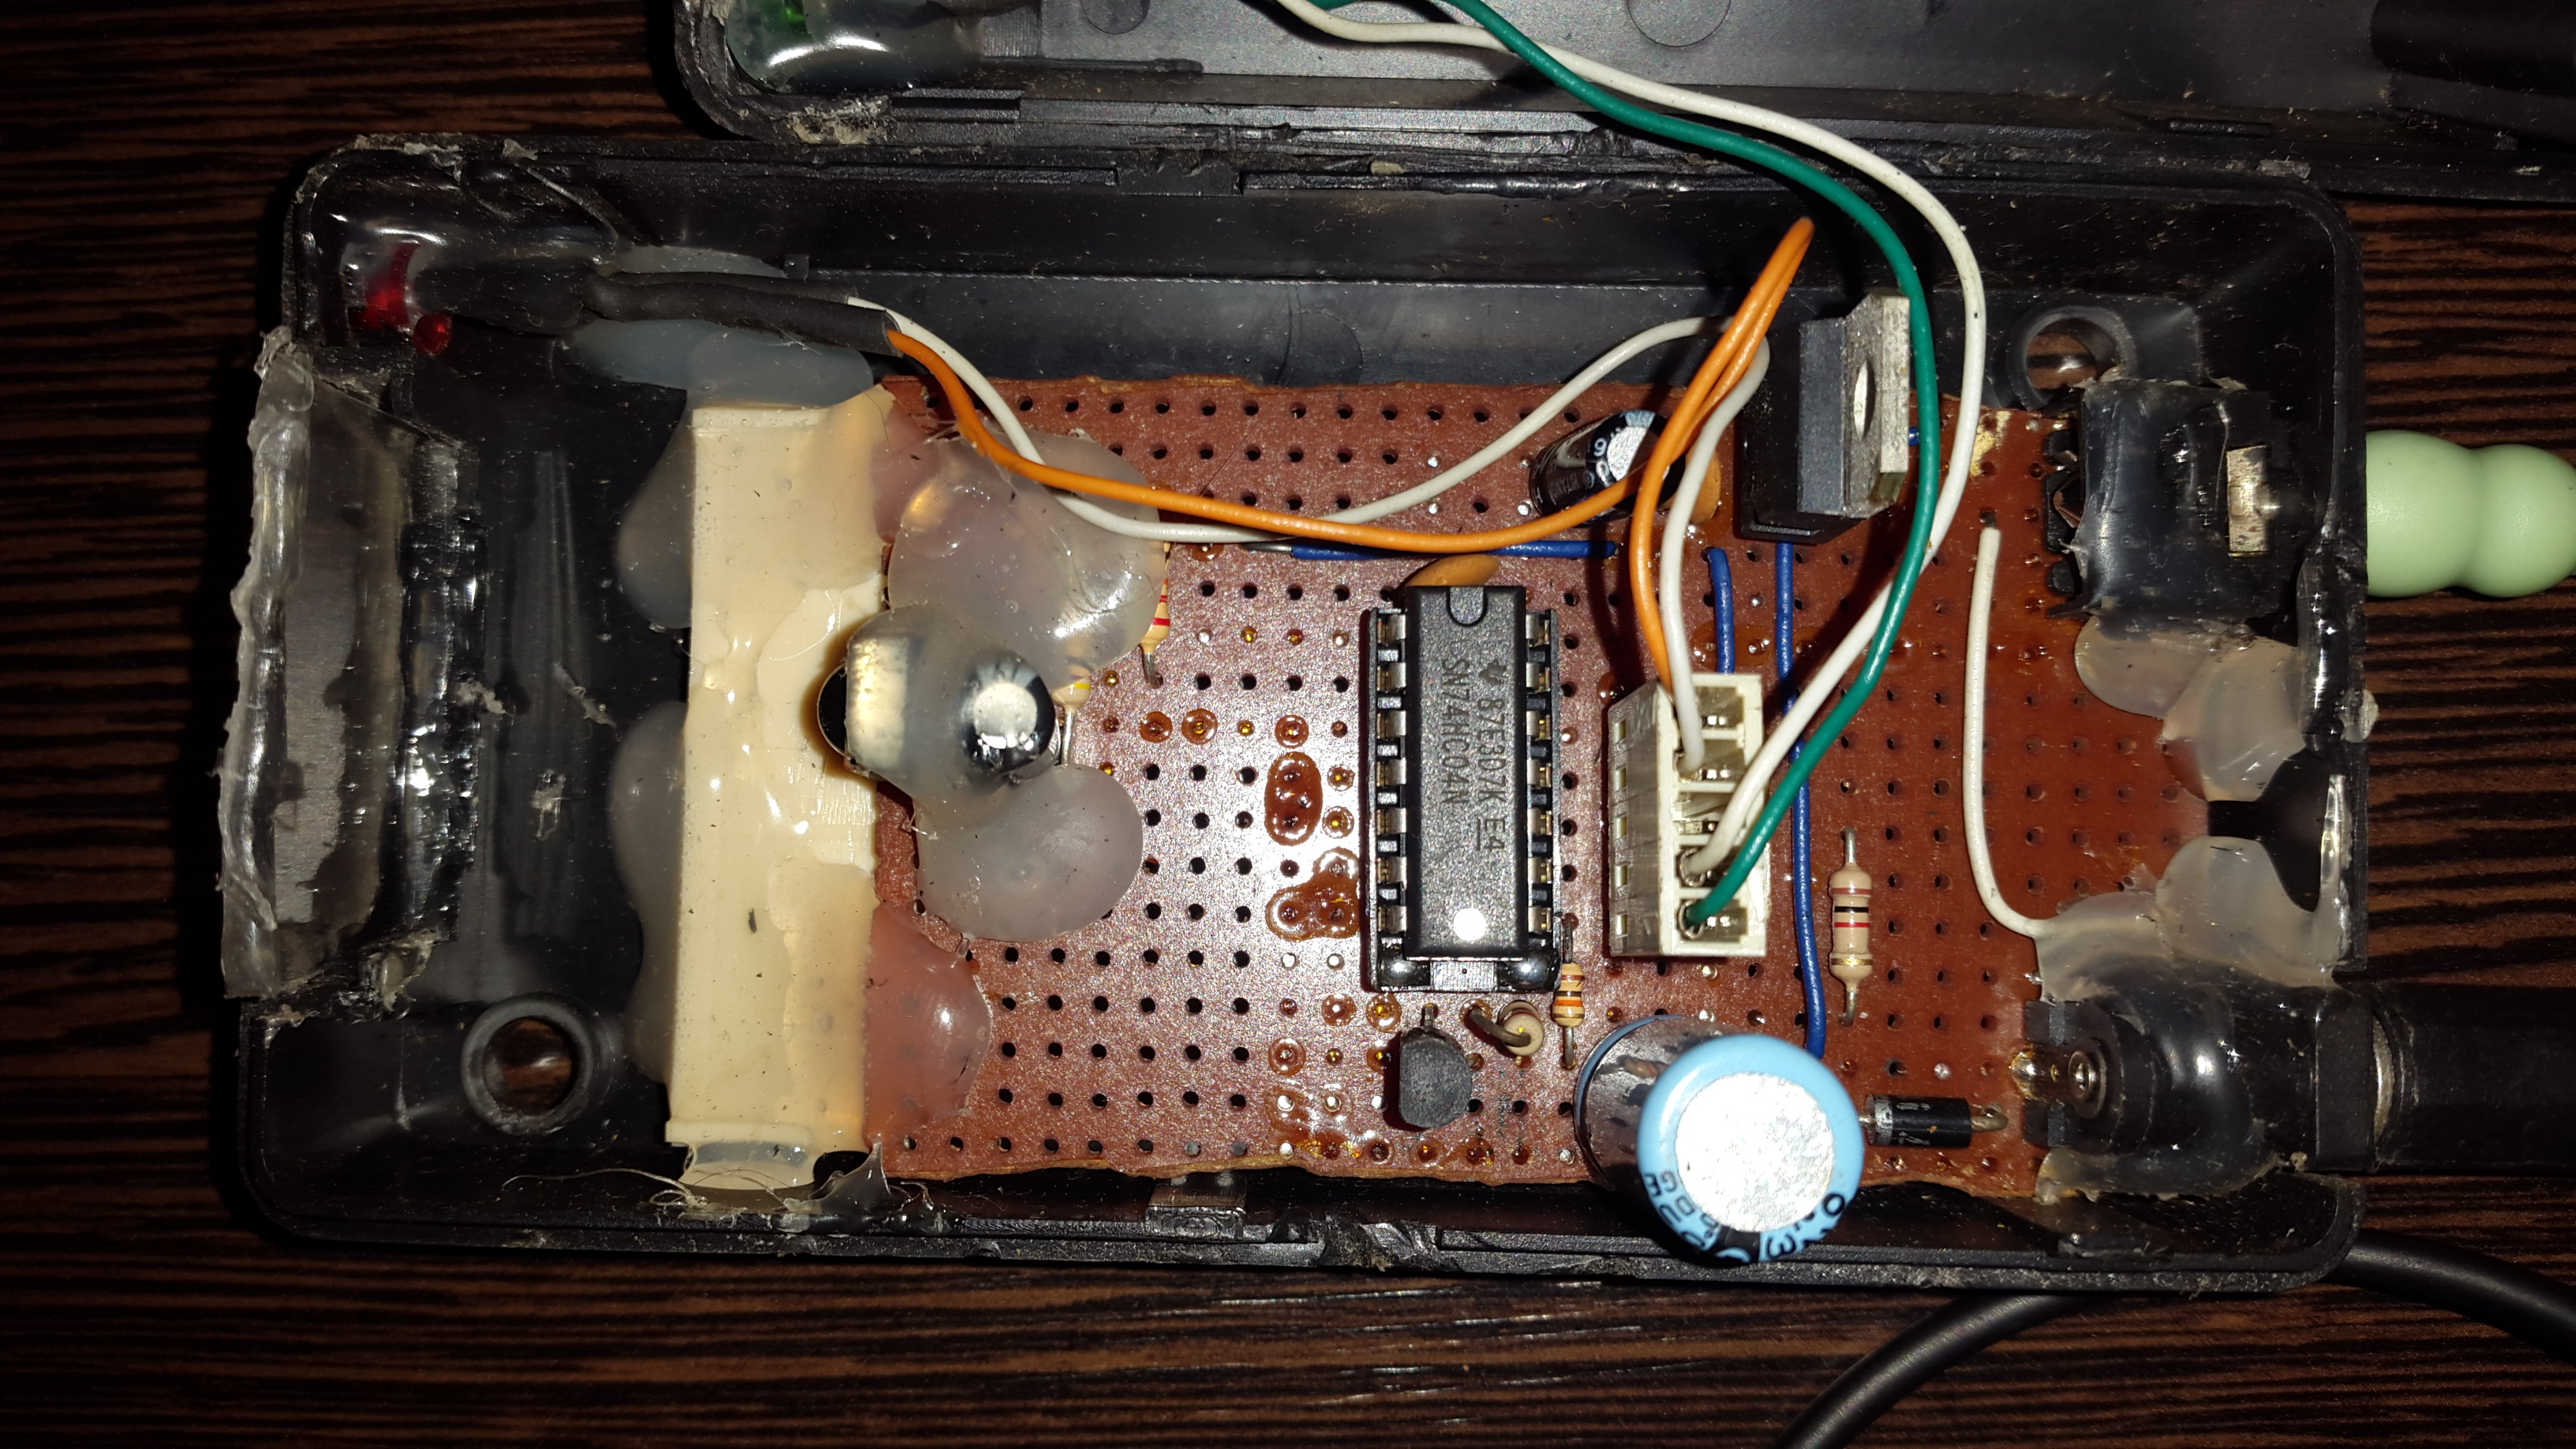
\includegraphics[width=0.9\paperwidth, angle=90]{img/REAL/receiver.jpg}
	\caption{\footnotesize{Receptor implementado.}}
	\label{fig:IR_receiver_real}
\end{figure}


\clearpage


\begin{figure}[H]
	\centering
	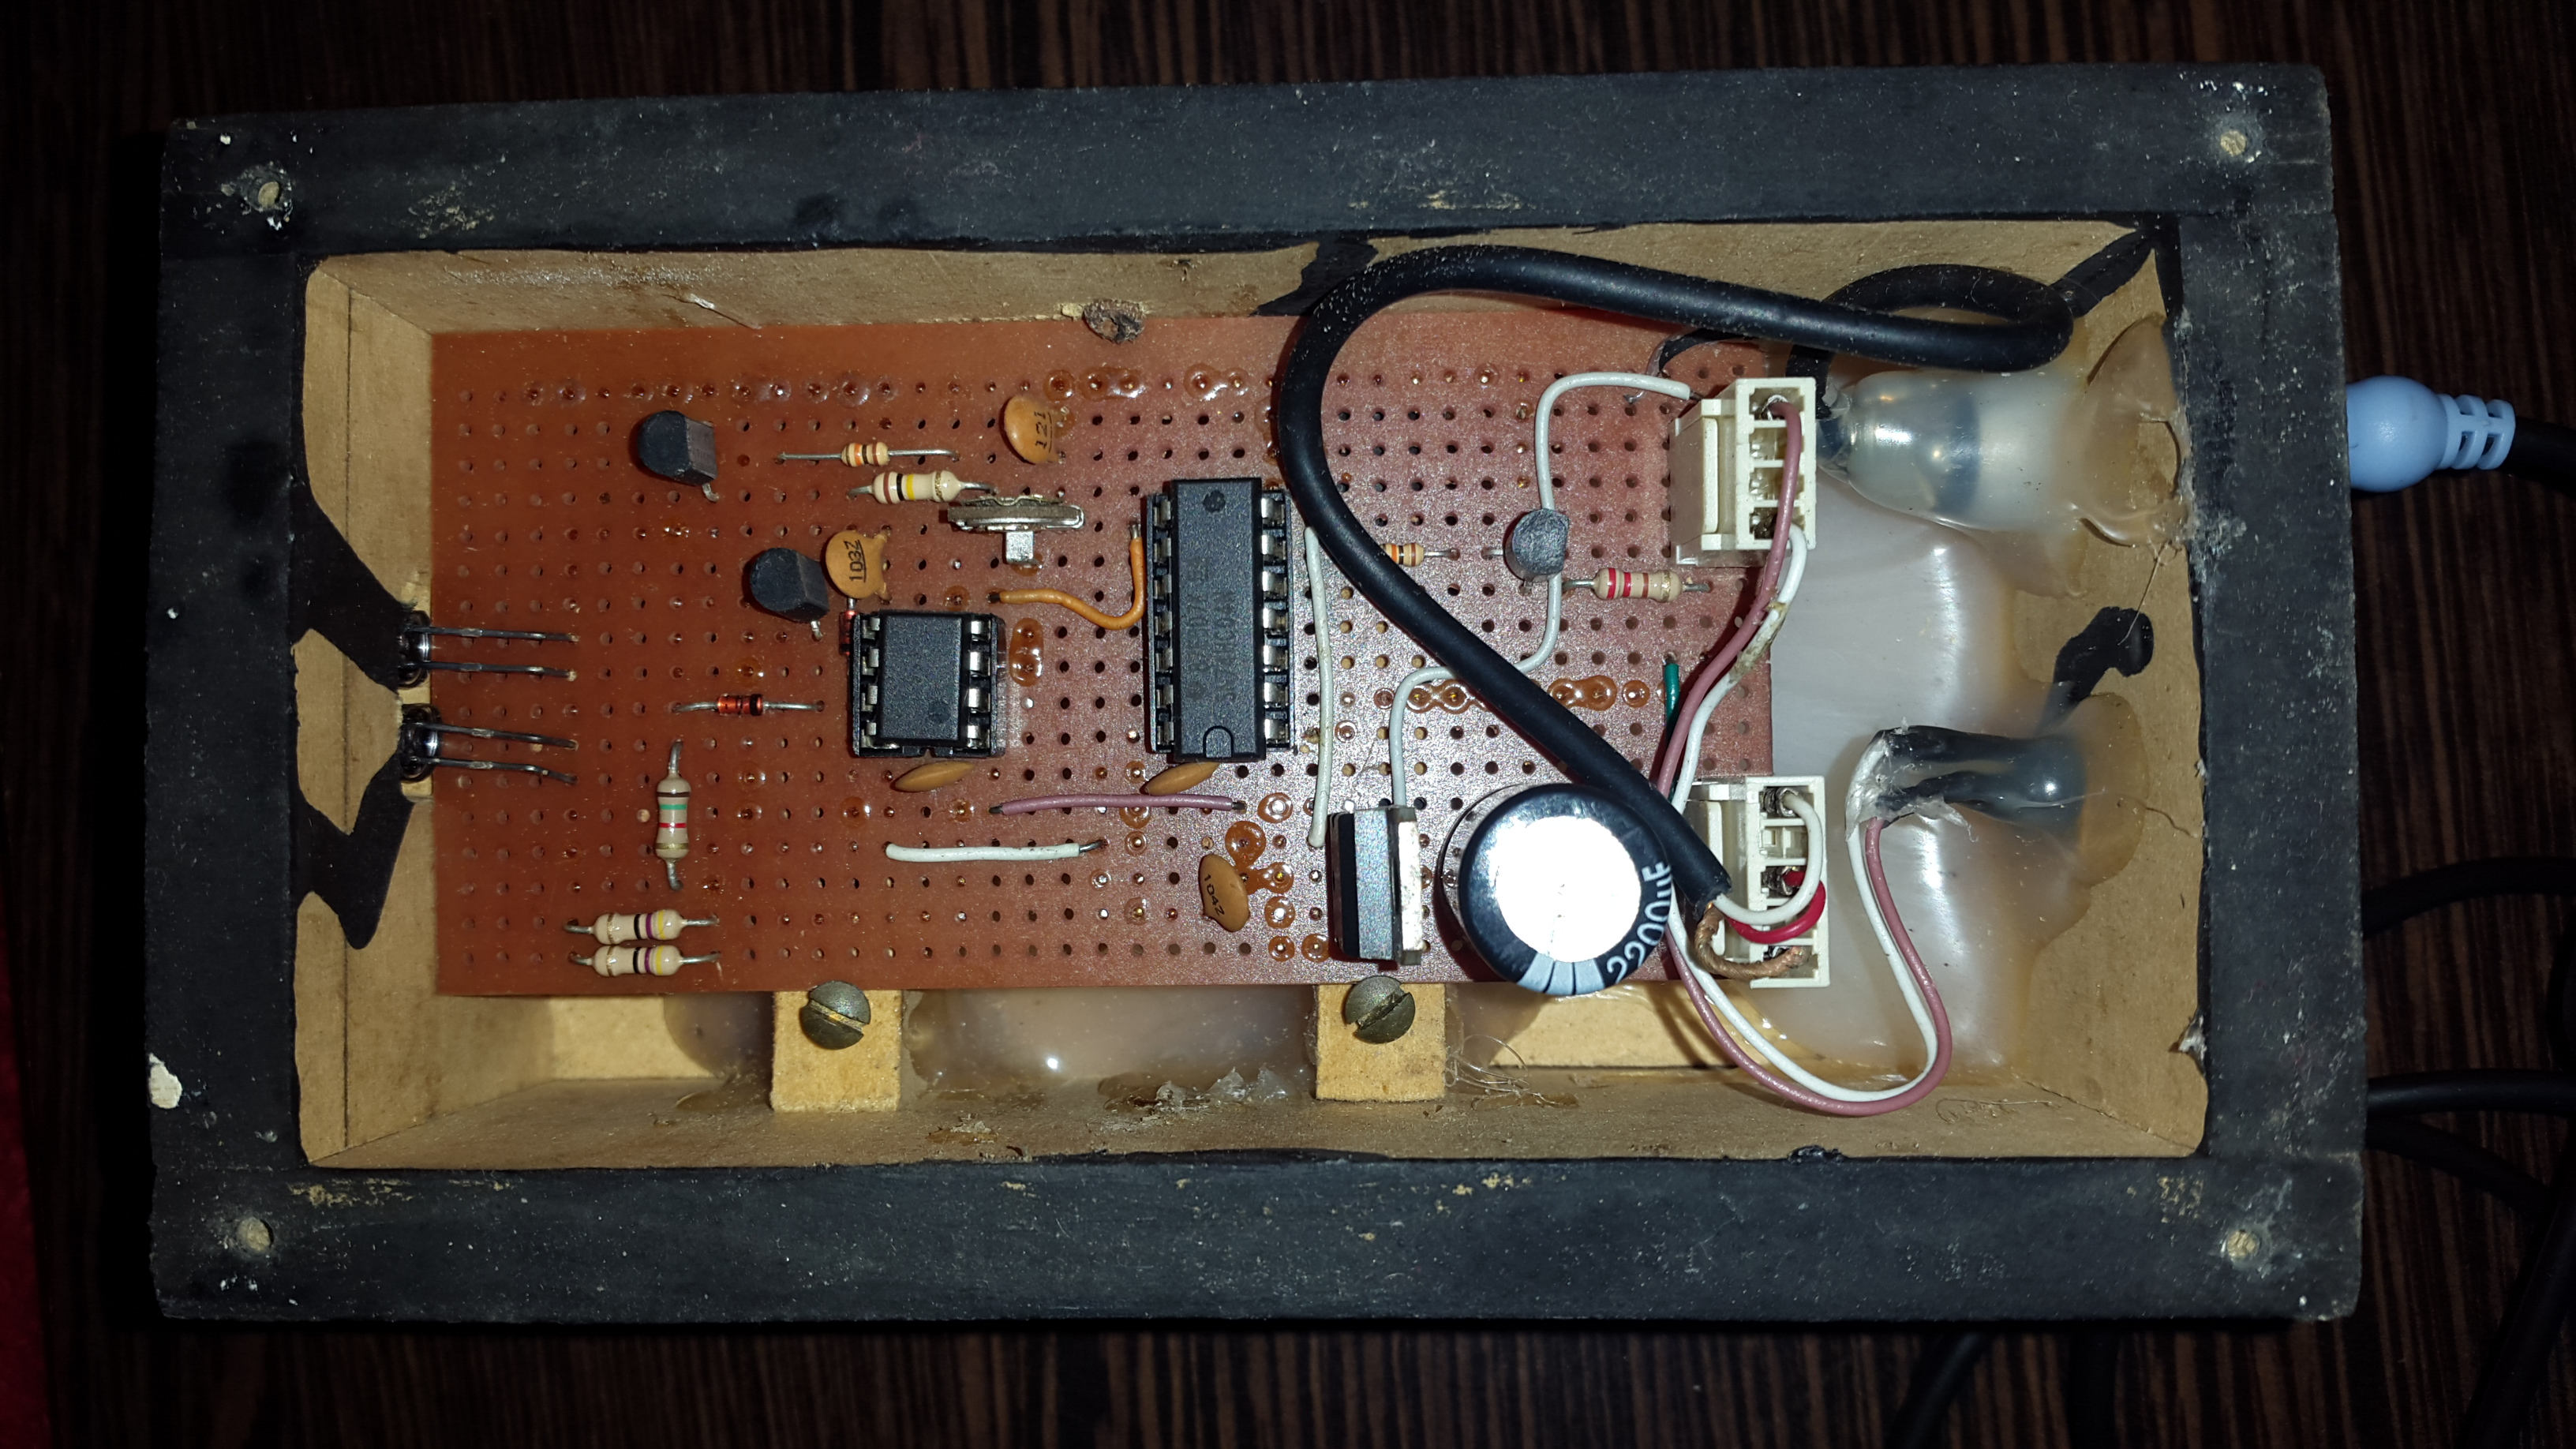
\includegraphics[width=0.9\paperwidth, angle=90]{img/REAL/transmitter.jpg}
	\caption{\footnotesize{Transmisor implementado.}}
	\label{fig:IR_transmitter_real}
\end{figure}


\clearpage


\begin{figure}[H]
	\centering
	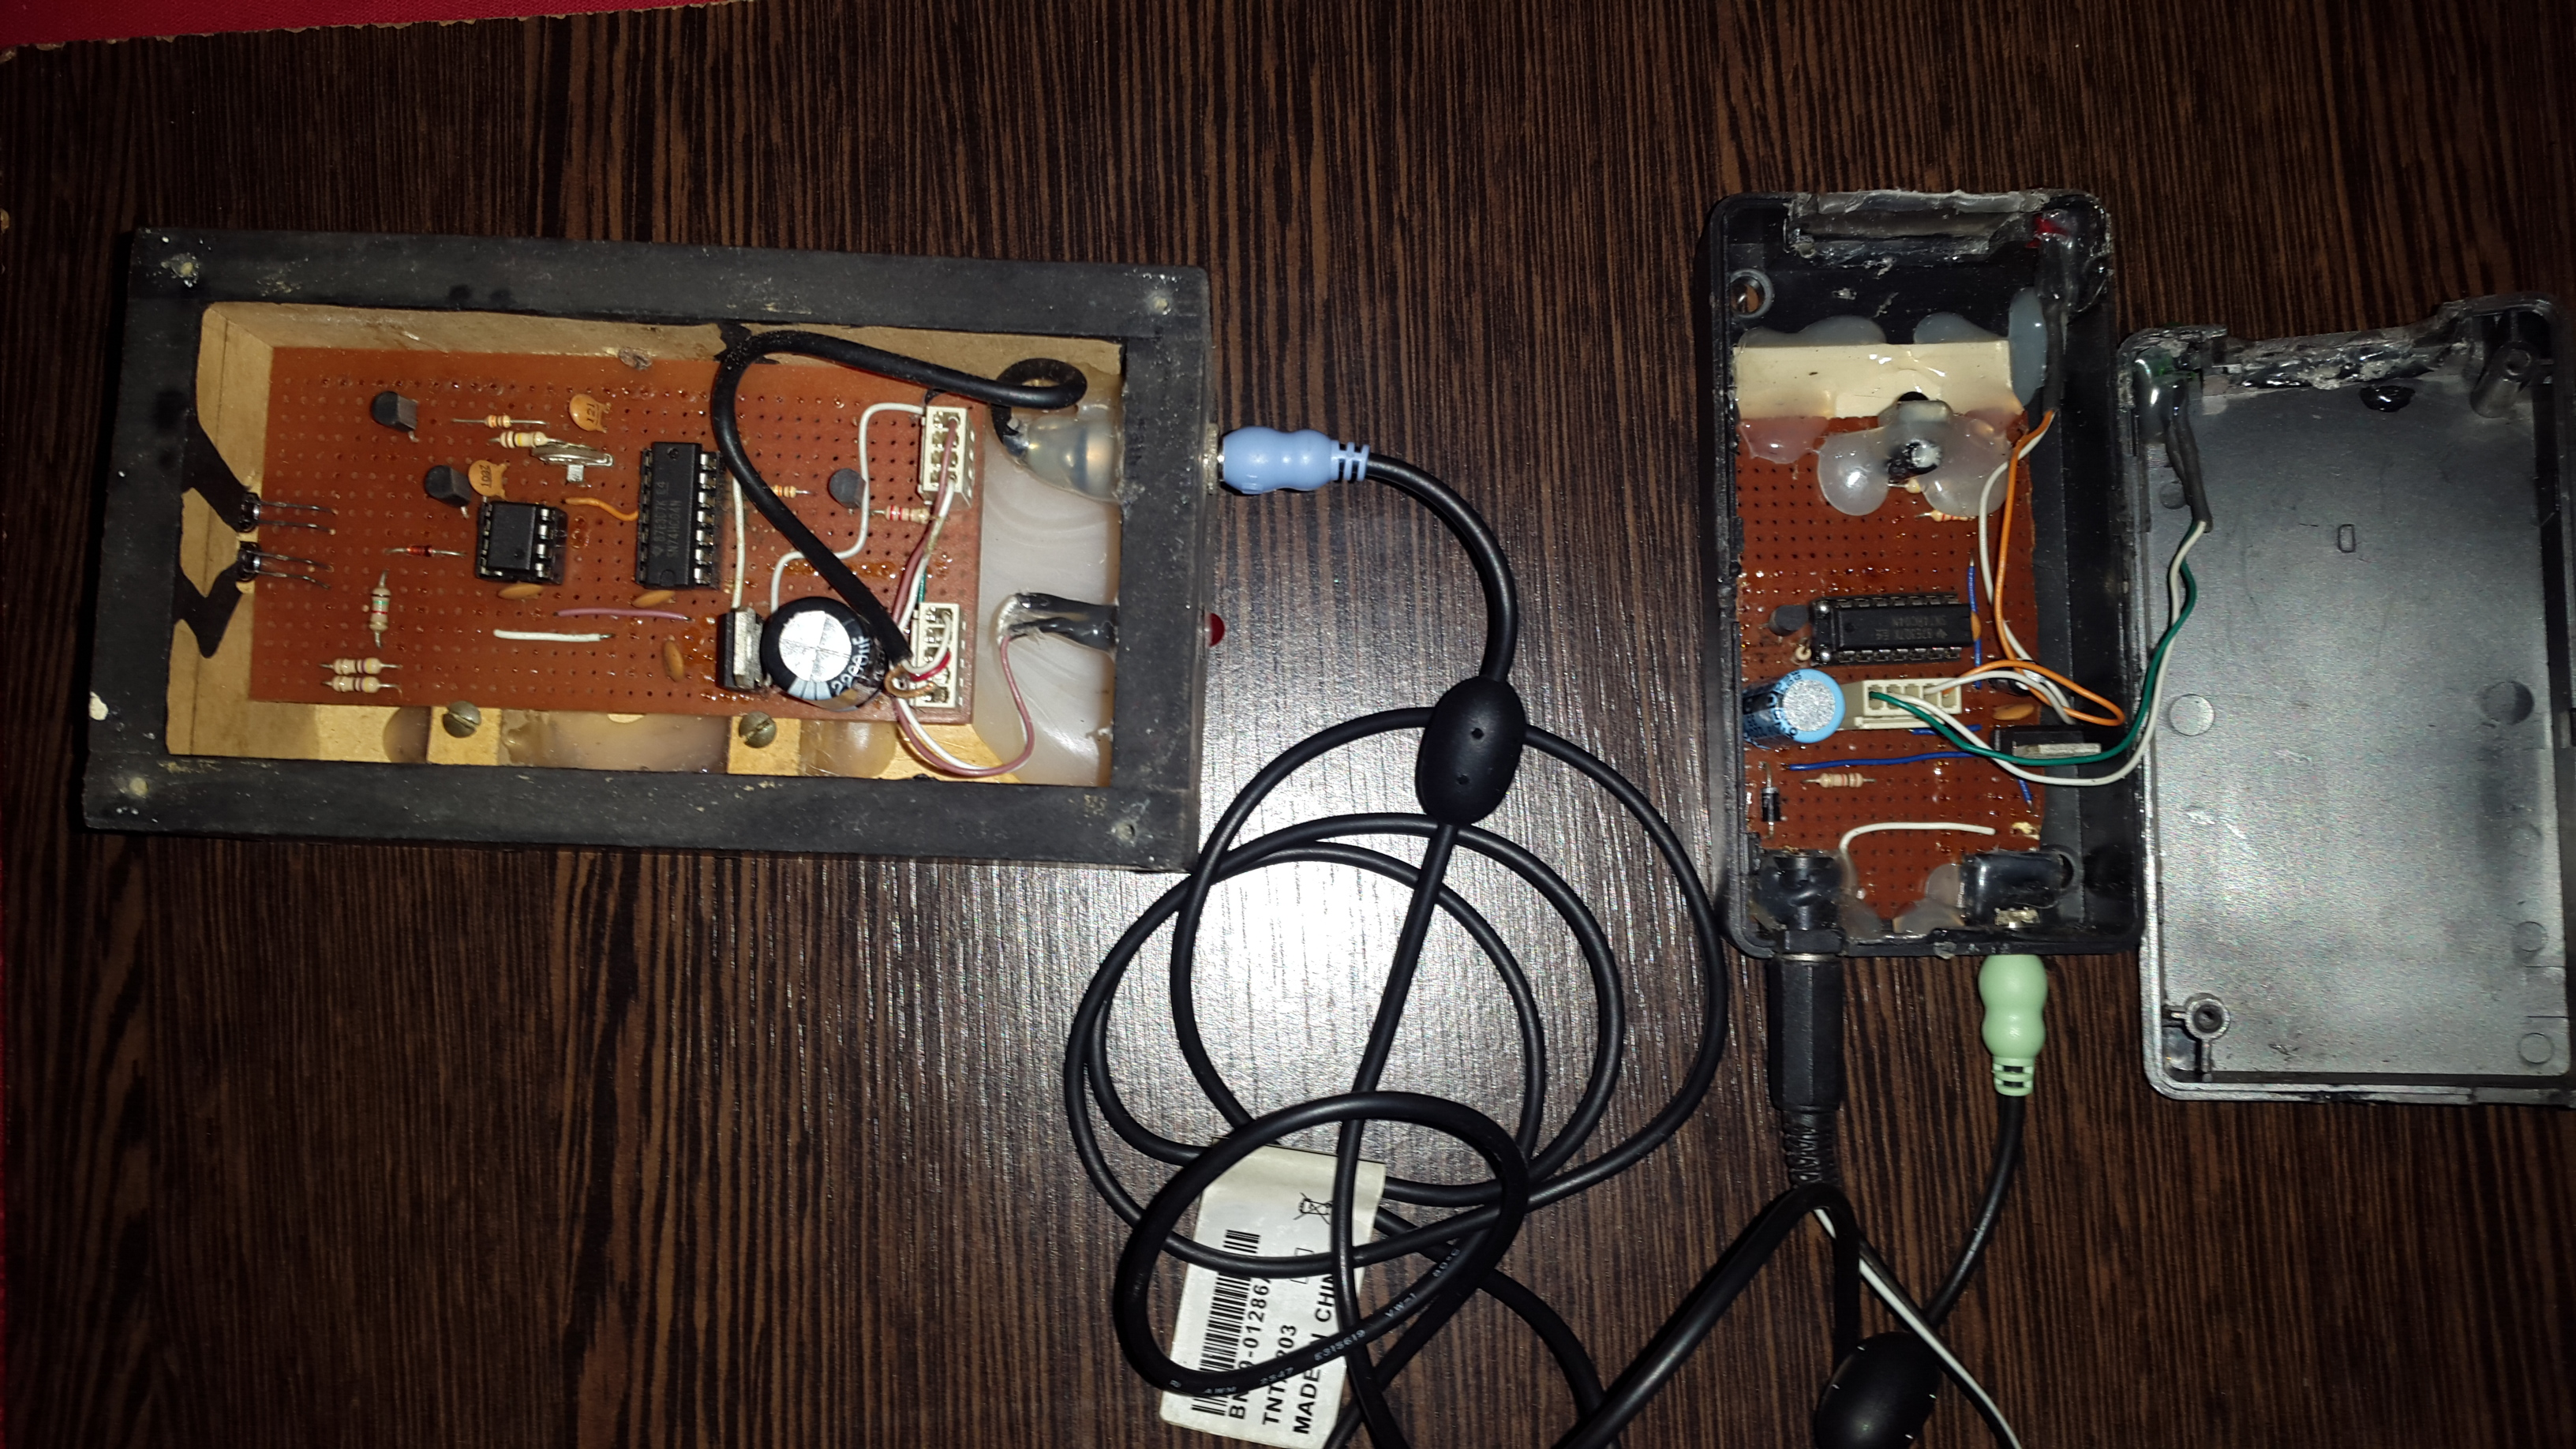
\includegraphics[width=0.9\paperwidth, angle=90]{img/REAL/complete.jpg}
	\caption{\footnotesize{Conexión de los módulos.}}
	\label{fig:IR_complete_real}
\end{figure}
